\chapter{Hoeffding Tree Ensembles}
\label{chap:improvebackground} 

In machine learning classification, an {\em ensemble} of classifiers is a
collection of several models combined together.
Algorithm~\ref{alg:genericensemble} lists a generic procedure for creating ensembles that is commonly used in batch learning.

\begin{algorithm}
\caption{Generic ensemble training algorithm.}
\begin{algorithmic}[1]
\STATE Given a set of training examples $S$
\FORALL{models $h_{m}$ in the ensemble of $M$ models, $m \in \{1,2,...,M\}$}
\STATE Assign a weight to each example in $S$ to create weight distribution $D_{m}$
\STATE Call {\bf base learner}, providing it with $S$ modified by weight distribution $D_{m}$ to create hypothesis $h_{m}$
\ENDFOR
\end{algorithmic}
\label{alg:genericensemble}
\end{algorithm}

This procedure requires three elements to create an ensemble:

\begin{enumerate}
\item A set $S$ of training examples
\item A {\em base} learning algorithm
\item A method of assigning weights to examples (line 3 of the pseudo-code)
\end{enumerate}

The third requirement, the weighting of examples, forms the major difference between ensemble methods. Another potential difference is the voting procedure. Typically each member of the
ensemble votes towards the prediction of class labels, where voting is either
{\em weighted} or {\em unweighted}. In weighted voting individual
classifiers have varying influence on the final combined vote,
the models that are believed to be more accurate will be trusted more than
those that are less accurate on average. In unweighted voting all models
have equal weight, and the final predicted class is the label
chosen by the majority of  ensemble members. Ensemble algorithms,
algorithms responsible for inducing an ensemble of models, are sometimes
known as {\em meta-learning} schemes. They perform a higher level of
learning that relies on lower-level {\em base} methods to produce the
individual models.

Ensemble methods are attractive because they can often be more accurate
than a single classifier alone. The best ensemble methods are modular,
capable of taking any base algorithm and improving its performance---any
method can be taken off the shelf and `plugged in'. Besides the added
memory and computational cost of sustaining multiple models, the main drawback
is loss of interpretability. A single decision tree may be easily
interpreted by humans, whereas the combined vote of several trees will be difficult to interpret.

In batch learning, cases where the base model is already difficult to
interpret or a {\em black-box} solution is acceptable, the potential for
improved accuracy easily justifies the use of ensembles where
possible. In the data stream setting, the memory and time requirements of
multiple models need more serious consideration. The demands of a data
stream application will be sensitive to the additive effect of
introducing more models, and there will be limits to the numbers of models
that can be supported. In limited memory learning---which is better, a single large model or many smaller models of equivalent combined size?

An ensemble of classifiers will be more accurate than any of its individual members if two conditions are met~\cite{nnensembles, tgensembles}. Firstly, the models must be accurate, that is, they must do better than random guessing. Secondly, they must be diverse, that is, their errors should not be correlated. If these conditions are satisfied Hansen and Salamon~\cite{nnensembles} show that as the number of ensemble members increase, the error of the ensemble will tend towards zero in the limit. The accuracy of an ensemble in practice will fall short of the improvement that is theoretically possible, mostly because the members which have been trained on variations of the same training data will never be completely independent.

Dietterich surveys ensemble methods for machine learning classification~\cite{dietterichensembles}. He mentions three possible reasons for the success of ensemble methods in practice: statistical, computational and representational. The {\em statistical} contribution to success is that the risk of incorrect classification is shared among multiple members, so that the average risk is lower than relying on a single member alone. The {\em computational} contribution is that more than one attempt is made to learn what could be a computationally intractable problem, where each attempt guided by heuristics could get stuck in local minima, but the average of several different attempts could better solve the problem than any individual attempt. The {\em representational} contribution is that an ensemble of models may be more capable of representing the true function in the data than any single model in isolation.

Decision trees are the basic machine learning model being investigated by this \thesisc, and they make an excellent base for ensemble methods, for several reasons given below. This is verified in practice,
where ensembles of decision trees are ranked among the best known methods
in contemporary machine learning~\cite{mlcomparison}.

The statistical reasoning and the uncorrelated errors theories both suggest that member diversity is crucial to good ensemble performance.
Ensemble methods typically exploit the lack of {\em stability} of a base
learner to increase diversity, thus achieve the desired effect of better accuracy in combination.
Breiman~\cite{bagging} defines {\em stable} methods as those not sensitive to small changes in training data---the more sensitive a method is to data changes the more {\em unstable} it is said to be.
Decision trees are good candidates for ensembles because they are
inherently unstable. The greedy local decisions can easily be influenced by only slight differences in training data, and the effect of a single change will be propagated to the entire subtree below. Naive Bayes in contrast is stable as it takes substantial differences in training data to modify its outcome.

In the stream setting, the nature of the Hoeffding bound decision
might suggest that Hoeffding trees may not exhibit such instability.
However, the bound only guides local per-split decisions---Domingos
and Hulten~\cite{vfdt} prove that overall the algorithm approximates the batch
induction of decision trees. The empirical results of the tree
ensembles in the next chapter demonstrate that Hoeffding trees are indeed unstable.

Decision trees also suit the computational argument. Computing an optimal decision tree is an NP-complete problem~\cite{optimaldtnp}, so out of necessity the algorithm performs a greedy local search. Several decision trees can approach the problem based on different searches involving local greedy decisions, which on average may form a better approximation of the true target than any single search.

\begin{figure}
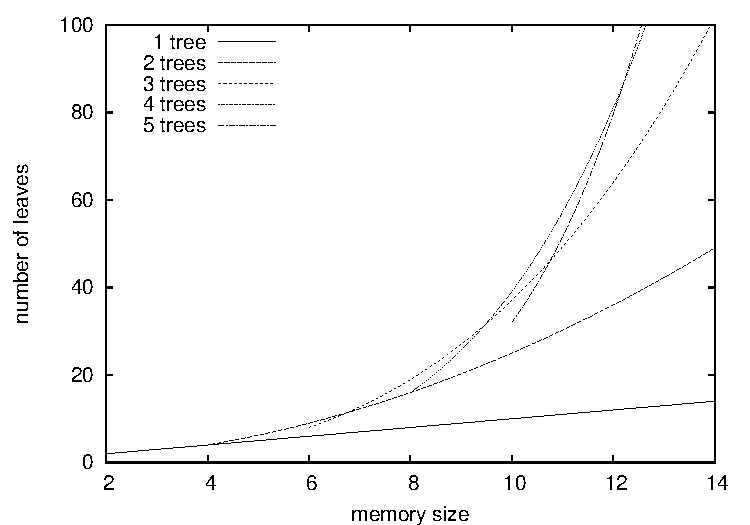
\includegraphics{figures/multitreereppower2}
\caption{A simple model of the leaf count of combinations of decision trees as a function of total memory size.}
\label{fig:multitreereppower}
\end{figure}

It is interesting to consider the representational argument applied to ensembles of decision trees, especially where memory is limited. In theory an ensemble of decision trees can be represented by a single standard decision tree, but the cost of constructing such a tree is expensive. Consider the process of combining two trees, $A$ and $B$. This can be achieved by replacing every leaf of $A$ with a subtree that is a complete copy of tree $B$, where the leaves copied from $B$ are merged with the leaf of $A$ that was replaced. Quinlan~\cite{miniboost} shows that the procedure is multiplicative, with only limited opportunity to simplify the resulting combined tree in most cases. 

Each leaf of a decision tree represents a particular region of the example space. The more leaves a tree has, the more regions are isolated by the tree, and the more potential it has to reduce error. So the number of leaves in a tree is in some way related to its ``representational power''. The tree multiplication argument above suggests that the effective number of leaves in an ensemble of $n$ trees, each having $l$ leaves, should be approximately $l^n$. 
Assume that the number of leaves that can be supported is a linear function of memory size $m$. Given that $m$ is fixed, the average number of leaves in individual trees in an ensemble of $n$ trees is at least two, and at most $m/n$. Combining these simplifying assumptions, the relative number of leaves in an ensemble of $n$ trees can be modeled by the function $(m/n)^n$, where $m/n \ge 2$. Figure~\ref{fig:multitreereppower} plots this function for ensemble sizes one to five. The figure shows for example that at memory size ten, an ensemble of three or four trees will effectively have more leaves than an ensemble of five trees, providing superior representation capacity.

These assumptions are unlikely to hold in practice. The leaf count of a tree is unlikely to be a perfect linear function of $m$, and it is also questionable whether the leaf count of tree combinations is perfectly multiplicative. The number of leaves will not directly translate into accuracy, which is obviously bounded and influenced by other factors. Despite these flaws the exercise demonstrates something useful about the expected behaviour of tree ensembles in limited memory---that a given number of combined trees will only be beneficial when sufficient memory is available, and the more trees involved, the more memory required. %Empirical evidence for this is found in Chapter~\ref{chap:improvecompare}.

A useful way to analyze ensemble behaviour is to consider the implications of {\em bias} and {\em variance}~\cite{bvdilemma, bvdecomp}. The typical formulation breaks the error of an algorithm into three parts:
\begin{equation} \label{eq:bvdecomp}
error = bias^2 + variance + noise
\end{equation}
Given a fixed learning problem, the first component of error is the {\em bias} of the machine learning algorithm, that is, how closely it matches the true function of the data on average over all theoretically possible training sets of a given size. The second error component is the {\em variance}, that is, how much the algorithm varies its model on different training sets of the given size. The third component of error is the intrinsic noise of the data, which an algorithm will not be able to overcome, thus setting an upper bound on the achievable accuracy. There is often a tradeoff between bias and variance, where reducing one can come at the expense of the other. Bias-variance decomposition~\cite{bvdecomp} is a tool that can help with understanding the behaviour of machine learning methods, and is discussed where appropriate throughout the chapter. %The discussion of results in Chapter~\ref{chap:improvecompare} uses empirical estimation of bias and variance to help with analysis.

The most common ensemble methods work like Algorithm~\ref{alg:genericensemble}, producing different models by manipulating the weight of each training example. This is why the stability of the base learner is significant. Other approaches that fall outside of this general model are not studied in this  \thesisc. They include removing attributes, such as attempted by Tumer and Ghosh~\cite{tgensembles}; manipulating the class labels, as used by Dietterich and Bakiri~\cite{ecoc} in their {\em error-correcting output codes} technique; and introducing randomness to the base model inducer, such as Breiman's popular {\em random forest} approach~\cite{randomforests}.

The following sections look at promising methods for improving accuracy, first in the batch setting (Section~\ref{sec:batchimprove}), followed by application to data streams (Section~\ref{sec:streamimprove}). 
First {\em bagging} (Sections~\ref{sec:baggingbatch} \&~\ref{sec:baggingstream}) and {\em boosting} (Section~\ref{sec:boostingbatch} \&~\ref{sec:boostingstream}) are investigated, then a third alternative, {\em option trees} (Section~\ref{sec:optiontreesbatch} \&~\ref{sec:hot}) are explored which offer a compromise between a single model and an ensemble of models.
Section~\ref{sec:enssizes} considers the numbers of ensemble members that can be supported in the batch and stream settings.

\section{Batch Setting}
\label{sec:batchimprove}

\subsection{Bagging}
\label{sec:baggingbatch}

Bagging ({\bf b}ootstrap {\bf agg}regat{\bf ing}) was introduced by Breiman~\cite{bagging}. The procedure is simple---it combines the unweighted vote of multiple classifiers, each of which is trained on a different {\em bootstrap replicate} of the training set. A bootstrap replicate is a set of examples drawn randomly {\em with replacement} from the original training data, to match the size of the original training data. The probability that any particular example in the original training data will be chosen for a random bootstrap replicate is 0.632, so each model in the ensemble will be trained on roughly 63.2\% of the full training set, and typically some examples are repeated several times to make the training size match the original.

Viewed in terms of the generic ensemble algorithm (Algorithm~\ref{alg:genericensemble}), in determining the weight distribution of examples for a particular model $D_{m}$ the weights will correspond to the number of times that an example is randomly drawn---those examples that are {\em out-of-bag} will have a weight of zero, while the majority are likely to have a pre-normalized weight of one, with those examples randomly selected more than once having a pre-normalized weight of more than one.

Bagging works best when the base algorithm is unstable, because the models produced will differ greatly in response to only minor changes in the training data, thus increasing the diversity of the ensemble. In terms of bias and variance, bagging greatly reduces the variance of a method, by averaging the diverse models into a single result. It does not directly target the bias at all, so methods whose variance is a significant component of error have the most to gain from this method.


\subsection{Boosting}
\label{sec:boostingbatch}

Boosting emerged from the field of {\em Computational Learning Theory}, a field that attempts to do mathematical analysis of learning. It tries to extract and formalize the essence of machine learning endeavours, with the hope of producing mathematically sound proofs about learning algorithms. The discovery and success of boosting shows that such efforts can positively impact the practical application of learning algorithms.

A framework that has become one of the main influences in the field is {\em PAC Learning} ({\bf P}robably {\bf A}pproximately {\bf C}orrect), proposed by Valiant~\cite{paclearn}.
Two concepts were defined by Kearns and Valiant~\cite{weakstronglearn}, the {\em strong} learner and the {\em weak} learner. A strong learner is one that is highly accurate. Formally, this is defined as a learner that given training examples drawn randomly from a binary concept space is capable of outputting a hypothesis with error no more than $\epsilon$, where $\epsilon > 0$, and does so with probability of at least $1 - \delta$, where $\delta > 0$. The defining requirement is that this must be achieved in runtime that is polynomial in all of 1/$\epsilon$, 1/$\delta$, and complexity of the target concept. A weak learner has the same requirements except that informally it needs only do slightly better than chance. Formally this means that in the weak case $\epsilon \le 1/2-\gamma$ where $0 < \gamma < 1/2$.

When these two notions of learning strength were introduced it was unknown whether the two are in fact equivalent, that is, whether a weak learner is also capable of strong learning. Schapire's paper ``The Strength of Weak Learnability''~\cite{strength} was the breakthrough that confirmed that this is indeed so. The paper shows that in the PAC framework weak learners are equivalent to strong learners by presenting an algorithm that is capable of ``boosting'' a weak learner in order to achieve high accuracy. Henceforth, the formal definition of a boosting algorithm is one that transforms a weak learner into a strong one.

Schapire's original hypothesis boosting algorithm works by combining many weak learners into a strong ensemble, as follows:

\begin{enumerate}
\item induce weak learner $h1$ as normal
\item train weak learner $h2$ with filtered examples, half of which $h1$ predicts correctly and the other half which $h1$ predicts incorrectly
\item train weak learner $h3$ only with examples that $h1$ and $h2$ disagree on
\item combine the predictions of $h1$, $h2$ and $h3$ by majority vote; if $h1$ and $h2$ agree then output the agreed upon class, otherwise output $h3$'s prediction
\end{enumerate}

Schapire proves with certain guarantees in the PAC framework that the combined vote of the hypotheses will be more accurate than $h1$ alone. By recursively applying this process, effectively creating a tree of hypotheses with three-way branches that are combined by majority vote (see left hand side of Figure~\ref{fig:boost_struct}), the weak learners can be progressively improved to form a classifier of combined weak hypotheses that is just as powerful as a single strong hypo \thesisc.

\begin{figure}
\centering
\begin{tabular}{c|c}
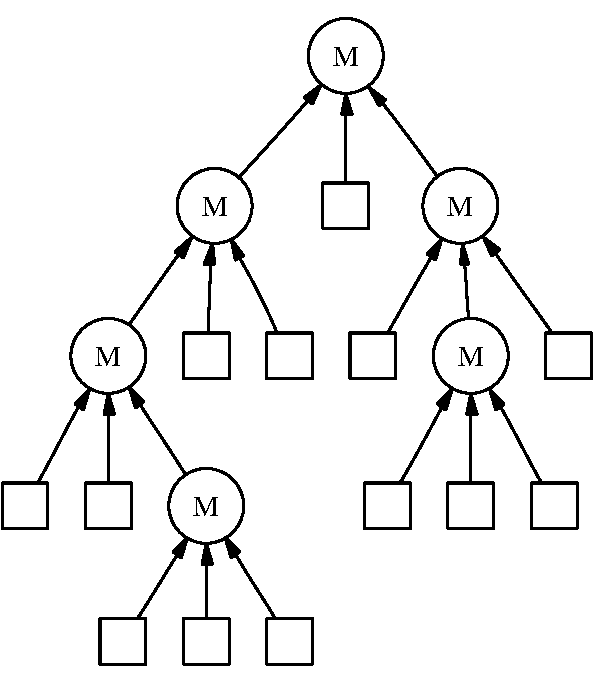
\includegraphics[width=0.40\textwidth]{figures/tree_boost} &
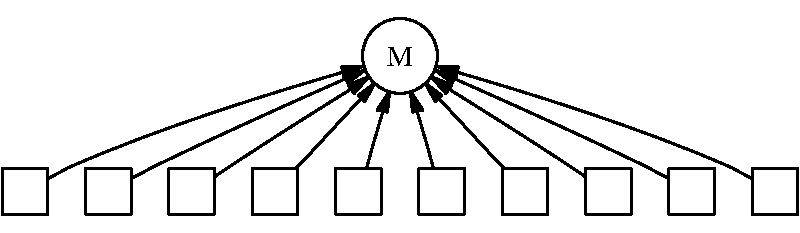
\includegraphics[width=0.55\textwidth]{figures/flat_boost} \\
\end{tabular}
\caption{Left hand side: recursive tree structure used by original hypothesis boosting. Right hand side: flat structure of {\em boost-by-majority} and AdaBoost.}
\label{fig:boost_struct}
\end{figure}

Schapire's work was improved by Freund~\cite{boostbymaj}, who presented an algorithm that is more efficient than Schapire's. In fact, Freund shows that the number of hypotheses needed for his {\em boost-by-majority} algorithm to reach a given accuracy is the smallest number possible. In this algorithm, the hypotheses are generated in a single flat level in sequence (see right hand side of Figure~\ref{fig:boost_struct}), as opposed to Schapire's recursive tree structure. The number of boosting iterations are fixed before induction begins, and there are two variants of the algorithm described, boosting by {\em sampling} and boosting by {\em filtering}.

Boosting by sampling is a method that suits the batch learning scenario. The first step of this process is to collect a training set from the concept space by requesting an entire batch of training examples, thus generating the set $S$. The goal of the process is then to create a hypothesis that is correct on all examples in $S$.
To do so, the most straightforward approach is to retain the entire set of $S$ in memory.

Boosting by filtering is a scenario that is more suited to incremental processing of data streams. There are interesting parallels between the theoretical learning situation proposed in the PAC framework and the challenges of data stream classification. This version of the algorithm works by selectively filtering the examples that are passed to the weak learners. The filter will either reject examples and discard them, or accept an example and pass it on to the appropriate weak learner. This variant has theoretical advantages over the sampling approach. In the filtering setting it is easier to analyze the expected amount of generalization that can be achieved, and the method can have superior space complexity due to not storing an entire training set.

The main problem with the {\em boost-by-majority} algorithm is that for it to work correctly the error ($\gamma$) of the weak learner must be known in advance. That is, how much better the base learner will perform over random guessing needs to be known before learning begins. This problem is serious enough to prevent the algorithm from being successful in practice.

The next advance in boosting algorithms was a combined effort of both Freund and Schapire~\cite{adaboost}. The {\em AdaBoost} algorithm adjusts {\bf ada}ptively to the errors of weak hypotheses, thus overcoming the problem of boosting by majority. The algorithm was introduced by taking an online allocation algorithm named {\em Hedge}, generalized from the {\em weighted majority algorithm}~\cite{wma}, and transforming it into a boosting algorithm. AdaBoost is a boosting by sampling method, and unfortunately a complementary filtering variant was not proposed. Limited to the sampling setting, it is shown that AdaBoost will drive training error exponentially towards zero in the number of iterations performed. AdaBoost is the most well known and successful boosting algorithm in practice. This is mostly due to it showing empirical evidence of accurately generalizing to data not included in the training set. Another reason for its popularity is that the algorithm is simple and intuitive. Freund and Schapire were awarded the 2003 G\"odel Prize for their work in recognition of the significant influence AdaBoost has had on the machine learning field and science in general.

\begin{algorithm}
\caption{AdaBoost. Input is a sequence of $m$ examples, {\bf WeakLearn} is the base weak learner and $T$ is the number of iterations.}
\begin{algorithmic}[1]
\STATE Initialize $D_{1}(i) = 1/m$ for all $i \in \{1,2,...,m\}$
\FOR{$t$ = 1,2,...$T$}
\STATE Call {\bf WeakLearn}, providing it with distribution $D_{t}$
\STATE Get back hypothesis $h_{t} : X \to Y$
\STATE Calculate error of $h_{t}: \epsilon_{t} = \sum_{i:h_{t}(x_{i}) \ne y_{i}} D_{t}(i)$
\IF{$\epsilon_{t} \ge 1/2$}
\STATE Set $T = t - 1$
\STATE Abort
\ENDIF
\STATE Set $\beta_{t} = \epsilon_{t} / (1 - \epsilon_{t})$
\STATE Update distribution $D_{t}: D_{t+1}(i) = \frac{D_{t}(i)}{Z_{t}} \times \left\{
\begin{array}{l l}
  \beta_{t} & \quad \mbox{if $h_{t}(x_{i}) = y_{i}$}\\
  1 & \quad \mbox{otherwise}\\
\end{array} \right.$
\\ where $Z_{t}$ is a normalization constant (chosen so $D_{t+1}$ is a probabilty distribution)
\ENDFOR
\RETURN final hypothesis: $h_{fin}(x) = \arg \max_{y \in Y} \sum_{t:h_{t}(x)=y} \log 1 / \beta_{t}$
\end{algorithmic}
\label{alg:adaboost}
\end{algorithm}

Algorithm~\ref{alg:adaboost} lists the AdaBoost pseudo-code. The intuitive understanding is that each new model in sequence will concentrate more on correctly classifying the examples that the previous models misclassified, and concentrate less on those that are already correct. To start with, all examples have equal weight (line 1). $T$ is the number of boosting iterations preformed. Every iteration starts by inducing a model on the data based on the weights currently assigned to examples, and the error, $\epsilon$, of the new model is estimated on the training data (lines 3-5). Lines 6-9 handle the special case where the error of the weak learner is worse than random guessing. A situation like this will confuse the weighting process so the algorithm aborts to avoid invalid behaviour. Lines 10-11 reweight the examples---those that are incorrectly classified retain their weight relative to correctly classified examples whose weight is reduced by $\frac{\epsilon}{1 - \epsilon}$, and the weights of all examples are normalized. The process repeats until a sequence of $T$ models have been induced.
To predict the class label of examples (line 13), each model in the final boosted sequence votes towards a classification, where each model's vote is weighted by $-\log \frac{\epsilon}{1 - \epsilon}$ so that models with lower error have higher influence on the final result.

The weak learner is influenced either by {\em reweighting} or {\em resampling} the training examples. Reweighting the examples requires that the weak learner respond to different continuous weights associated with each example. Common learners such as C4.5 and Naive Bayes have this capability. Resampling involves randomly sampling a new training set from the original according to the weight distribution. The advantage of resampling is that the weak learner need not handle continuous example weights, but the resampling approach introduces a random element to the process. When Breiman~\cite{arcing} compared the approaches he found that accuracy did not significantly differ between the two. 

Breiman looked at AdaBoost from a different perspective~\cite{arcing}. He introduced his own terminology, describing the procedure as {\em arcing} ({\bf a}daptively {\bf r}esample and {\bf c}ombine), and refers to AdaBoost as {\em arc-fs} (for {\bf F}reund and {\bf S}chapire). He found arc-fs to be very promising and capable of significantly outperforming bagging. As an exercise to test his theory that AdaBoost's success is due to the general adaptive resampling approach and not dependent on the precise formulation of arc-fs, he introduced a simpler ad-hoc algorithm, {\em arc-x4}, listed in Algorithm~\ref{alg:arc-x4}. The main differences from AdaBoost are:
\begin{enumerate}
\item A simpler weight update step. Each example is relatively weighted by $1+e^{4}$ where $e$ is the number of misclassifications made on the example by the existing ensemble.
\item Voting is unweighted.
\end{enumerate}
In experimental comparison~\cite{arcing}, arc-x4 performed on a comparable level to arc-fs. Both were often more successful than bagging at reducing test set error.

\begin{algorithm}
\caption{Arc-x4, Breiman's ad-hoc boosting algorithm.}
\begin{algorithmic}[1]
\STATE Initialize $D_{1}(i) = 1/m$ for all $i \in \{1,2,...,m\}$
\FOR{$t$ = 1,2,...$T$}
\STATE Call {\bf WeakLearn}, providing it with distribution $D_{t}$
\STATE Get back hypothesis $h_{t} : X \to Y$
\STATE Count misclassifications: $e_{i} = \sum_{n=1}^{t} I(h_{n}(x_{i}) \ne y_{i})$
\STATE Update distribution $D_{t}: D_{t+1}(i) = \frac{1+e_{i}^{4}}{\sum_{n=1}^{m} 1+e_{n}^4}$
\ENDFOR
\RETURN final hypothesis: $h_{fin}(x) = \arg \max_{y \in Y} \sum_{t=1}^{T} I(h_{t}(x) = y)$
\end{algorithmic}
\label{alg:arc-x4}
\end{algorithm}

Breiman~\cite{arcing} employs bias and variance analysis as a tool to help explain how boosting works. Whereas bagging reduces mostly variance, boosting has the ability to reduce both bias and variance. An intuitive understanding of boosting's ability to reduce bias is that subsequent boosting iterations have an opportunity to correct the bias of previous models in the ensemble. Breiman was still puzzled by some aspects of the behaviour of boosting, prompting deeper investigation by Freund and Schapire~\cite{arcingdiscuss}.

It is accepted and understood how AdaBoost reduces error on the training set, but uncertainty remains as to why error on test examples, the {\em generalization} error, continues to decrease after training set error reaches zero. Researchers including Breiman were surprised at AdaBoost's ability to generalize well beyond any theoretical explanations and seemingly in contradiction to {\em Occam's razor}, which suggests that simpler solutions should be preferred over more complex ones. Schapire and Freund et al.~\cite{boostingmargin} tried to explain this phenomenon in their paper ``Boosting the Margin: A New Explanation for the Effectiveness of Voting Methods''. They suggest that the {\em margin} of the predictions, the difference between the confidence of the true class and the confidence of the highest other class, continues to improve with additional boosting iterations, explaining the ability to improve generalization. However the uncertainty continues, as Breiman~\cite{arcingresponse, breimanpredgames} provides contrary evidence and claims that the margin explanation is incomplete. The true explanation for AdaBoost's generalization ability remains uncertain, but this of course does not prevent its use in practice.

The statisticians Friedman, Hastie and Tibshirani~\cite{logitboost} point out the
similarities between AdaBoost and {\em additive logistic regression}, a
more established and commonly understood statistical technique. From an
optimization point of view they show that AdaBoost performs gradient
descent in function space that aims to minimise the following {\em
exponential loss} function:
\begin{equation} \label{eq:exploss}
\exp \left( -y_{i} \sum_{t=1}^{T} \alpha h_{t}(x_{i}) \right)
\end{equation}
Friedman et al. question why exponential loss is used, suggesting other
possibilities, and propose a boosting variant named {\em LogitBoost}. Their insight has provided another perspective on AdaBoost,
which further aids researchers in understanding its workings. Another
contribution they provide is the idea of {\em weight trimming}---after
several boosting iterations there can exist examples with very low weight,
so low in fact that ignoring them will not harm accuracy while reducing
computation.

Schapire and Singer~\cite{boostimproved} make further improvements to AdaBoost. The original formulation only used binary votes of ensemble members to
reweight examples. The improved formulation generalizes the algorithm to
make use of confidences output by base members, potentially improving
performance. They show how to handle multiple class labels and also study how to best devise algorithms to output confidences suiting the improved AdaBoost. Additionally, they propose an alternative gain criterion, so that for example, decision trees can be induced that aim to directly improve boosting performance.

Early enthusiasm for AdaBoost sometimes overlooked its shortcomings. Observing its spectacular ability to generalize on many data sets it was
sometimes suggested that AdaBoost is resistant to overfitting.
Dietterich~\cite{boostnoise} addressed such claims by demonstrating that AdaBoost can suffer from problems with noise. In fact, his experiments show that
with substantial classification noise, bagging is much better than
boosting. The explanation for this behaviour is that AdaBoost will
inevitably give higher weight to noisy examples, because they will
consistently be misclassified.

An interesting piece of follow-up work was conducted by Freund~\cite{brownboost}, who revisited his {\em boost-by-majority} algorithm to make it adaptive like AdaBoost. The result is the {\em BrownBoost} algorithm. BrownBoost considers the limit in which each boosting iteration makes an infinitesimally small contribution to the whole process, which can be modelled with {\it {\bf Brown}ian motion}. As with the original boost-by-majority, the number of iterations, $T$, is fixed in advance. The algorithm is optimized to minimize the training error in the pre-assigned number of iterations---as the final iteration draws near, the algorithm
gives up on examples that are consistently misclassified. This offers hope
of overcoming the problems with noise that are suffered by AdaBoost. In
fact, Freund shows that AdaBoost is a special case of BrownBoost, where $T
\to \infty$. Despite the theoretical benefits of BrownBoost it has
failed to draw much attention from the community, perhaps because it is
much more complicated and less intuitive than AdaBoost. The study~\cite{boost3exp} found that BrownBoost is more robust than AdaBoost in class noise, but that LogitBoost performs at a comparable level.


\subsection{Option Trees}
\label{sec:optiontreesbatch}

Standard decision trees have only a single path that each example can follow\footnote{For simplicity, this statement ignores missing value approaches such as C4.5 that send examples down several paths when testing on unknown attribute values.}, so any given example will apply to only one leaf in the tree. Option trees, introduced by Buntine~\cite{buntinetrees} and further explored by Kohavi and Kunz~\cite{kohaviot}, are more general, making it possible for an example to travel down multiple paths and arrive at multiple leaves. This is achieved by introducing the possibility of {\em option nodes} to the tree, alongside the standard decision nodes and leaf nodes. An option node splits the decision path several ways---when an option node is encountered several different subtrees are traversed, which could themselves contain more option nodes, thus the potential for reaching different leaves is multiplied by every option. Making a decision with an option tree involves combining the predictions of the applicable leaves into a final result.

Option trees are a single general structure that can represent anything from a single standard decision tree to an ensemble of standard decision trees to an even more general tree containing options within options. An option tree without any option nodes is clearly the same as a standard decision tree. An option tree with only a single option node at the root can represent an ensemble of standard trees. Option nodes below other option nodes take this a step further and have the combinational power to represent many possible decision trees in a single compact structure.

A potential benefit of option trees over a traditional ensemble is that the more flexible representation can save space---consider as an extreme example an ensemble of one hundred mostly identical large trees, where the only difference between each tree lies at a single leaf node, in the same position in each tree. The standard ensemble representation would require one hundred whole copies of the tree where only the leaf would differ. Efficiently represented as an option tree this would require almost a hundred times less space, where the varying leaf could be replaced by an option node splitting one hundred ways leading to the one hundred different leaf variants. The drive for diverse ensembles will of course make such a scenario unlikely, but the illustration serves the point that there are savings to be made by combining different tree permutations into a single structure. Essentially every path above an option node can be saved from repetition in memory, compared to explicitly storing every individual tree found in combination.

Another possible benefit offered by option trees is retention of interpretability. An accepted disadvantage of ensemble methods is that users will lose the ability to understand the models produced. An option tree is a single structure, and in some situations this can aid in interpreting the decision process, much more so than trying to determine the workings of several completely separate models in combination. An option tree containing many options at many levels can be complex, but humans may not be as confused by a limited number of option nodes in small and simple option trees. Arguments for the interpretability of option trees can be found in~\cite{kohaviot,adtrees}.

In terms of accuracy, an option tree is just as capable of increasing accuracy as any ensemble technique. Depending on how it is induced, an option tree could represent the result of bagging or boosting trees, or something else entirely. An example application of boosting to option tree induction is the {\em alternating decision tree} (ADTree) learning algorithm by Freund and Mason~\cite{adtrees}.

The option tree induction approach by Kohavi and Kunz~\cite{kohaviot} seeks to explore and average additional split possibilities that a tree could make. Their approach is closer to bagging than boosting, because bagging also draws out different possibilities from the trees, but operates in a random and less direct fashion. It is less like boosting because it does not utilize classification performance as feedback for improving on previous decisions, but blindly tries out promising-looking paths that have previously not been explored. They provide two main reasons why such trees should outperform a single decision tree, {\em stability} and {\em limited lookahead}. The stability argument has already been discussed with other ensemble methods---a single tree can differ wildly on small changes in training data, but an option tree that combines several possibilities would vary less on average. The limited lookahead argument refers to the fact that standard decision trees make greedy local decisions, and do not consider better decisions that could be made if the search looked ahead before committing. Looking ahead is expensive and studies suggest that looking ahead a few steps is futile~\cite{dtlookahead}, but when the tree considers attributes in isolation it will be unaware of potential interactions between attributes that could greatly increase accuracy. By exploring several alternative options, an option tree increases the chance of utilizing rewarding attribute combinations.

A significant difficulty with inducing option trees is that they will grow very rapidly if not controlled. This is due to their powerful combinatorial nature which gives them high representational power, but which can also easily explore too many options if left unchecked. Kohavi and Kunz employ several strategies to prevent a combinatorial explosion of possibilities. Firstly, they set a parameter that controls how close other tests must be to the best test to be considered as extra options. The larger the {\em option factor}, the more potential there is for additional options to be explored. Secondly, they impose an arbitrary limit of five options per node. Because this is enforced locally per node, it will slow down but not completely prevent excessive combinations. Thirdly, they experimented with restricting splits to certain depths of the tree, either the lowest three levels or the top two levels, and also tried altering the frequency of options as a function number of supporting examples or tree depth.

Kohavi and Kunz~\cite{kohaviot} compared their option trees to bagged trees in experiments, showing that option trees are superior.
Their hypothesis was that options nearer the root are more useful than options further down the tree, which was confirmed in their experiments. Interestingly, this opinion differs from that of Buntine~\cite{buntinetrees}, who argued that options are more effective nearer the leaves.

\section{Data Stream Setting}
\label{sec:streamimprove}

\subsection{Bagging}
\label{sec:baggingstream}

Bagging as formulated by Breiman does not seem immediately applicable to data streams, because it appears that the entire data set is needed in order to construct bootstrap replicates. Oza and Russell~\cite{ozabagboost} show how the process of sampling bootstrap replicates from training data can be simulated in a data stream context. They observe that the probability that any individual example will be chosen for a replicate is governed by a {\em Binomial} distribution, so the sampling process can be approximated by considering each example in turn and randomly deciding with a Binomial probability distribution how many times to include the example in the formation of a replicate set. The difficulty with this solution is that the number of examples, $N$, needs to be known in advance. Oza and Russell get around this by considering what happens when $N \to \infty$, which is a reasonable assumption to make with data streams of arbitrary length, and conclude that the Binomial distribution tends to a {\em Poisson}(1) distribution. Following these observations the algorithm is straightforward to implement, listed in Algorithm~\ref{alg:ozabag}. It requires a base learner that is also capable of processing data streams.

\begin{algorithm}
\caption{Oza and Russell's {\em Online Bagging}. $M$ is the number of models in the ensemble and $I(\cdot)$ is the indicator function.}
\begin{algorithmic}[1]
\STATE Initialize base models $h_{m}$ for all $m \in \{1,2,...,M\}$
\FORALL{training examples}
\FOR{$m=1,2,...,M$}
\STATE Set $k = $ {\em Poisson}(1)
\FOR{$n=1,2,...,k$}
\STATE Update $h_{m}$ with the current example
\ENDFOR
\ENDFOR
\ENDFOR
\STATE {\bf anytime output:}
\RETURN hypothesis: $h_{fin}(x) = \arg \max_{y \in Y} \sum_{t=1}^{T} I(h_{t}(x) = y)$
\end{algorithmic}
\label{alg:ozabag}
\end{algorithm}

Oza and Russell construct proofs to demonstrate that their ``online'' bagging algorithm converges towards the original batch algorithm~\cite{ozabagboost}, and have collected experimental evidence to show this~\cite{ozaexp}. One issue they have not addressed is memory management, a consideration that is paramount in this  \thesisc. Assuming that a memory-limited base algorithm is available, such as the Hoeffding tree algorithm studied in Chapter~\ref{chap:hoeffdingtrees}, then the memory requirements of an ensemble of trees can be controlled by limits on individual members. The experimental implementation of bagged Hoeffding trees takes a simple approach to controlling total memory usage---with an overall memory limit of $m$ and a total of $n$ trees, each tree is limited to a maximum size of $m/n$.


\subsection{Boosting} 
\label{sec:boostingstream}

Existing literature for the problem of applying boosting to data stream
classification has mainly focussed on modifying AdaBoost, and often under the guise of {\em online} learning~\cite{ozabagboost, fszboost}. 
The term ``online'' is slightly ambiguous, as researchers have used it in the past to refer to varying goals. Typically the focus is on processing a single example at a time, but sometimes without emphasis on other factors believed important in this \thesis  such as memory and time requirements.
For the most part however the online methods reviewed here are directly applicable to the data stream setting.
Attempts at modifying boosting to work in an ``online'' fashion can be
divided into two main approaches: {\em block} boosting and {\em parallel}
boosting.

Block boosting involves collecting data from the stream into sequential blocks,
reweighting the examples in each block in the spirit of AdaBoost, and then
training a batch learner to produce new models for inclusion in the
ensemble. An advantage of this approach is that specialized data stream
based learners are not required, the boosting ``wrapper'' algorithm
handles the data stream. Memory management by such a method can be
achieved by discarding weaker models, but this raises
interesting questions---traditional AdaBoost depends on the previous set
of ensemble members remaining constant, the effect of removing arbitrary
models from an ensemble during learning is unknown. Margineantu and Dietterich~\cite{pruneboost} look at pruning models from AdaBoost ensembles and find it effective, although they do this after learning is complete. A significant difficulty with block boosting is deciding how large the blocks should be. A demanding batch learner and/or overly large block sizes will limit the rate at which examples can be processed, and block sizes that are too small will limit accuracy.
Examples of block boosting include Breiman's pasting of `bites'~\cite{pastingbites}, and the study by Fan et al.~\cite{fszboost}.

Parallel boosting involves feeding examples as they arrive into a base data stream algorithm that builds each ensemble member in parallel. A difficulty is that AdaBoost was conceived as a sequential process. Sequential weighting of training examples can be simulated by feeding and reweighting examples through each member in sequence. This does not directly emulate the
strictly sequential process of AdaBoost, as models further down the
sequence will start learning from weights that depend on earlier models
that are also evolving over time, but the hope is that in time the
models will converge towards an AdaBoost-like configuration. An advantage
of using data stream algorithms as base learners is that the ensemble
algorithm can inherit the ability to adequately handle data stream demands.

Examples of parallel boosting include Fern and Givan's~\cite{branchpred} online adaptation of arc-x4, and Domingo and Watanabe's~\cite{madaboost} {\em MadaBoost}. Domingo and Watanabe describe difficulties with correctly weighting examples when applying AdaBoost to the online setting. Their solution is essentially to put a limit on the highest weight that can be assigned to an example. They try to prove that their modification is still boosting in the formal PAC-learning sense but face theoretical problems that prevent them from providing a full proof. Bshouty and Gavinsky~\cite{polyboost} present a more theoretically sound solution to the problem, performing {\em polynomially smooth} boosting, but the result is far less intuitive than most AdaBoost-like algorithms.

\begin{algorithm}
\caption{Oza and Russell's {\em Online Boosting}. $N$ is the number of examples seen.}
\begin{algorithmic}[1]
\STATE Initialize base models $h_{m}$ for all $m \in \{1,2,...,M\}, \lambda_{m}^{sc}=0, \lambda_{m}^{sw}=0$
\FORALL{training examples}
\STATE Set ``weight'' of example $\lambda_{d} = 1$
\FOR{$m=1,2,...,M$}
\STATE Set $k = $ {\em Poisson}($\lambda_{d}$)
\FOR{$n=1,2,...,k$}
\STATE Update $h_{m}$ with the current example
\ENDFOR
\IF{$h_{m}$ correctly classifies the example}
\STATE $\lambda_{m}^{sc} \gets \lambda_{m}^{sc} + \lambda_{d}$
\STATE $\lambda_{d} \gets \lambda_{d} \left( \frac{N}{2 \lambda_{m}^{sc}} \right)$
\ELSE
\STATE $\lambda_{m}^{sw} \gets \lambda_{m}^{sw} + \lambda_{d}$
\STATE $\lambda_{d} \gets \lambda_{d} \left( \frac{N}{2 \lambda_{m}^{sw}} \right)$
\ENDIF
\ENDFOR
\ENDFOR
\STATE {\bf anytime output:}
\STATE Calculate $\epsilon_{m} = \frac{\lambda_{m}^{sw}}{\lambda_{m}^{sc} + \lambda_{m}^{sw}}$ and $\beta_{m} = \epsilon_{m} / (1 - \epsilon_{m})$ for all $m \in \{1,2,...,M\}$
\RETURN hypothesis: $h_{fin}(x) = \arg \max_{y \in Y} \sum_{m:h_{m}(x)=y} \log 1 / \beta_{m}$
\end{algorithmic}
\label{alg:ozaboost}
\end{algorithm}

The data stream boosting approach adopted by this \thesis  is a parallel boosting algorithm that was developed by Oza and Russell~\cite{ozabagboost}, who compliment their online bagging algorithm (Section~\ref{sec:baggingstream}) with a similar approach to online boosting. The pseudo-code is listed in Algorithm~\ref{alg:ozaboost}.
Oza and Russell note that the weighting procedure of AdaBoost actually divides the total example weight into two halves---half of the weight is assigned to the correctly classified examples, and the other half goes to the misclassified examples. As the ensemble gets more accurate the number of misclassified examples should progressively get less and less relative to the number of correct classifications. In turn, the misclassified set gets more weight per example than the correctly classified set. This motivates the weight update procedure in lines 9-15, which is intended to simulate the batch weight behaviour in a streaming environment, much like the online bagging algorithm is designed to simulate the creation of bootstrap replicates. Once again they utilize the Poisson distribution for deciding the random probability that an example is used for training, only this time the parameter ($\lambda_{d}$) changes according to the boosting weight of the example as it is passed through each model in sequence. The use of random Poisson is well founded for bagging, but motivation for it in the boosting situation is less clear. Preliminary experimental work for this \thesis  involved testing several boosting algorithms, including a modification of Oza and Russell's boosting algorithm that applied example weights directly instead of relying on random drawings from Poisson. Overall the algorithm performed better {\em with} the random Poisson element than without it, so it seems to be a worthwhile approach even if the theoretical underpinning is weak.

%Of the boosting strategies tested in preliminary experimentation, Oza and Russell's approach represents the best found. 
%More discussion about the performance of boosting in data streams is reserved for Section~\ref{sec:boostdiscuss}.
% As with bagging, the memory management strategy tested in Chapter~\ref{chap:improvecompare} uses the simple approach of controlling total ensemble size by enforcing uniform memory limits to each base tree.


\subsection{Option Trees} 
\label{sec:hot}

A new algorithm for inducing option trees from data streams was devised for this  \thesisc. It is based on the Hoeffding tree induction algorithm, but generalized to explore additional options in a manner similar to the option trees of Kohavi and Kunz~\cite{kohaviot}. The pseudo-code is listed in Algorithm~\ref{alg:hot}. The algorithm is an extension of the basic decision tree inducer listed in Algorithm~\ref{alg:ht} on page~\pageref{alg:ht}. The differences are, firstly, that each training example can update a set of option nodes rather than just a single leaf, and secondly, lines 20-32 constitute new logic that applies when a split has already been chosen but extra options are still being considered.

\begin{algorithm}
\caption{Hoeffding option tree induction algorithm. $\delta'$ is the confidence for additional splits and $maxOptions$ is the maximum number of options that should be reachable by any single example.}
\begin{algorithmic}[1]
\STATE Let $HOT$ be an option tree with a single leaf (the root)
\FORALL{training examples}
\STATE Sort example into leaves/option nodes $L$ using $HOT$
\FORALL{option nodes $l$ of the set $L$}
\STATE Update sufficient statistics in $l$
\STATE Increment $n_l$, the number of examples seen at $l$
\IF{$n_l$ $mod$ $n_{min}$ $= 0$ {\bf and} examples seen at $l$ not all of same class}
\IF{$l$ has no children}
\STATE Compute $\overline{G}_{l}(X_{i})$ for each attribute
\STATE Let $X_{a}$ be attribute with highest $\overline{G}_{l}$
\STATE Let $X_{b}$ be attribute with second-highest $\overline{G}_{l}$
\STATE Compute Hoeffding bound $\epsilon = \sqrt{\frac{R^{2}ln(1/\delta)}{2n_{l}}}$
\IF{$X_{a} \ne X_{\emptyset}$ {\bf and} ($\overline{G}_{l}(X_{a}) - \overline{G}_{l}(X_{b}) > \epsilon$ {\bf or} $\epsilon < \tau$)}
\STATE Add a node below $l$ that splits on $X_{a}$
\FORALL{branches of the split}
\STATE Add a new option leaf with initialized sufficient statistics
\ENDFOR
\ENDIF
\ELSE
\IF{$optionCount_{l} < maxOptions$}
\STATE Compute $\overline{G}_{l}(X_{i})$ for existing splits and (non-used) attributes
\STATE Let $S$ be existing child split with highest $\overline{G}_{l}$
\STATE Let $X$ be (non-used) attribute with highest $\overline{G}_{l}$
\STATE Compute Hoeffding bound $\epsilon = \sqrt{\frac{R^{2}ln(1/\delta')}{2n_{l}}}$
\IF{$\overline{G}_{l}(X) - \overline{G}_{l}(S) > \epsilon$}
\STATE Add an additional child option to $l$ that splits on $X$
\FORALL{branches of the split}
\STATE Add a new option leaf with initialized sufficient statistics
\ENDFOR
\ENDIF
\ELSE
\STATE Remove attribute statistics stored at $l$
\ENDIF
\ENDIF
\ENDIF
\ENDFOR
\ENDFOR
\end{algorithmic}
\label{alg:hot}
\end{algorithm}

A minor point of difference between Kohavi and Kunz's option tree and the Hoeffding option trees implemented for this study is that the Hoeffding option tree uses the class confidences in each leaf to help form the majority decision. The observed probabilities of each class are added together, rather than the binary voting process used by Kohavi and Kunz where each leaf votes completely towards the local majority in determining the overall majority label. Preliminary experiments suggested that using confidences in voting can slightly improve accuracy.

Just as Kohavi and Kunz needed to restrict the growth of their option trees in the batch setting, strategies are required to control the growth of Hoeffding option trees. Without any restrictions the tree will try to explore all possible tree configurations simultaneously which is clearly not feasible.

The first main approach to controlling growth involves the initial decision of when to introduce new options to the tree. Kohavi and Kunz have an {\em option factor} parameter that controls the inducer's eagerness to add new options. The Hoeffding option tree algorithm has a similar parameter, $\delta'$, which can be thought of as a secondary Hoeffding bound confidence. The $\delta'$ parameter controls the confidence of secondary split decisions much like $\delta$ influences the initial split decision, only for additional splits 
the test is whether the information gain of the best candidate exceeds the information gain of the best split already present in the tree.
For the initial split, the decision process searches for the best attribute overall, but for subsequent splits, the search is for attributes that are superior to existing splits. It is very unlikely that any other attribute could compete so well with the best attribute already chosen that it could beat it by the same initial margin. Recall, the original Hoeffding bound decision is designed to guarantee that the other attributes should not be any better. For this reason, the secondary bound $\delta'$ needs to be much looser than the initial bound $\delta$ for there to be any chance of additional attribute choices.
It seems a contradiction to require other attributes to be better when the Hoeffding bound has already guaranteed with high confidence that they are not as good, but the guarantees are much weaker when tie breaking has been employed, and setting a sufficiently loose secondary bound does indeed create further split options.
$\delta'$ can be expressed in terms of a multiplication factor $\alpha$, specifying a fraction of the original Hoeffding bound:
\begin{equation}
\delta' = e^{\alpha ^ 2 \ln(\delta)}
\label{eq:deltaprime1}
\end{equation}
Or equivalently:
\begin{equation}
\alpha = \sqrt{\frac{\ln(\delta')}{\ln(\delta)}}
\label{eq:deltaprime2}
\end{equation}
For example, with the default parameter settings of $\delta=10^{-7}$ and $\delta'=0.999$ then from Equation~\ref{eq:deltaprime2}, $\alpha \approx 0.0079$, that is, decisions to explore additional attributes are approximately 126 times more eager than the initial choice of attribute. Preliminary experiments found that a setting of $\delta'=0.999$ works well in combination with the second overriding growth strategy discussed next.

The second main approach to controlling tree growth involves directly limiting the number of options that the tree will explore. Kohavi and Kunz tried a local limit, where they would not allow an option node to split more than five different ways. This \thesis  introduces a global limiting strategy that instead of limiting options {\em per node} it limits options {\em per example}.  
A combinatorial explosion is still possible with a locally applied limit, whereas a global limit prevents it altogether.
Doing so requires more work to compute how many leaves are reachable at a particular point in the tree, and only allowing more options if it does not exceed the maximum allowed. Line 20 of Algorithm~\ref{alg:hot} performs the test that determines whether more options are possible, and assumes that the maximum reachability count ($optionCount_{l}$) of the node is available. Computing maximum reachability counts in an option tree is complicated---it not only depends on the descendants of a node but also on its ancestors, and their descendants too. To solve this problem an incremental algorithm was devised to keep track of maximum counts in each option node in the tree, listed in Algorithm~\ref{alg:hotcounter}. The worst-case complexity of this algorithm is linear in the number of nodes in the tree, as it could potentially visit every node once. All nodes start with an {\em optionCount} of 1. The operation for updating counts is employed every time the tree grows. 
Nodes are not removed from the tree, as pruning is not considered in this  \thesisc. However, an operation for removing option nodes, that would be needed if the option trees were pruned, is included for completeness.

\begin{algorithm}
\caption{Option counter update, for adding and removing options.}
\begin{algorithmic}
\STATE $\mathbf{Procedure} \, AddOption(node, newOption)$:
\STATE $max \gets node.optionCount$
\IF{$node$ has children}
\STATE $max \gets max+1$
\ENDIF
\FORALL{children of $newOption$}
\STATE $child.optionCount \gets max$
\ENDFOR
\STATE add $newOption$ as child of $node$
\STATE call UpdateOptionCount($node$,$newOption$)
\STATE
\STATE $\mathbf{Procedure} \, RemoveOption(node, index)$:
\WHILE{there are options below $node$}
\STATE remove deepest option
\ENDWHILE
\STATE remove child at $index$ from node
\STATE call UpdateOptionCountBelow($node$,-1)
\IF{$node$ has parent}
\STATE call UpdateOptionCount($parent$,$node$)
\ENDIF
\STATE
\STATE $\mathbf{Procedure} \, UpdateOptionCount(node, source)$:
\STATE $max \gets$ maximum $optionCount$ of $node$ children
\STATE $\delta \gets max - node.optionCount$
\IF{$\delta \neq 0$}
\STATE $node.optionCount \gets node.optionCount + \delta$
\FORALL{children of $node$ such that $child \neq source$}
\STATE call UpdateOptionCountBelow($child$,$\delta$)
\ENDFOR
\IF{$node$ has parent}
\STATE call UpdateOptionCount($parent$,$node$)
\ENDIF
\ENDIF
\STATE
\STATE $\mathbf{Procedure} \, UpdateOptionCountBelow(node, \delta)$:
\STATE $node.optionCount \gets node.optionCount + \delta$
\FORALL{children of $node$}
\STATE call UpdateOptionCountBelow($child$, $\delta$)
\ENDFOR
\end{algorithmic}
\label{alg:hotcounter}
\end{algorithm}

Interestingly, the arbitrary local limit of five options employed by Kohavi and Kunz also seems to be a good choice for the global limit suggested here, at least when memory restrictions are not considered. Early experiments looked at the effect of the {\em maxOptions} parameter on smaller scale runs in unbounded memory. The average accuracy across many data sets is plotted in Figure~\ref{fig:maxOptionAcc}, showing that prior to a maximum of five options there are significant accuracy gains, but after that point the accuracy gains diminish. The computational demands continue to rise with each additional option.

\begin{figure}
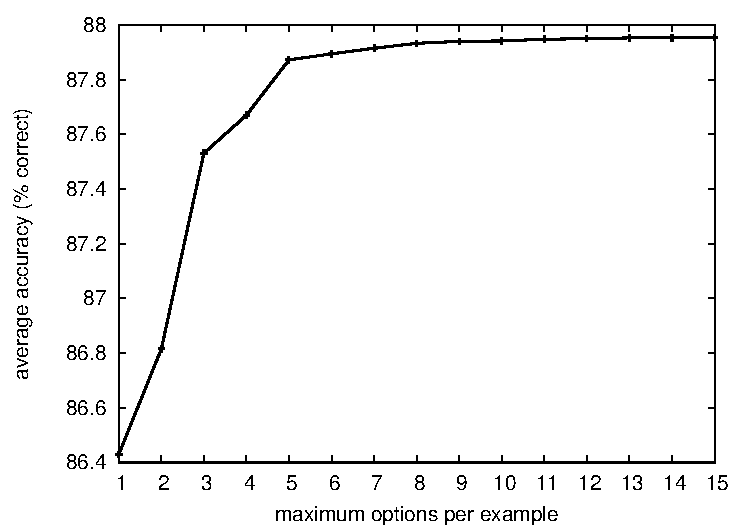
\includegraphics{figures/maxOptionAcc}
\caption{Average accuracy of Hoeffding option tree over many data sets versus the maximum number of options per example. Accuracies were estimated in unbounded memory.}
\label{fig:maxOptionAcc}
\end{figure}

Other design decisions also help to limit tree growth. When searching for additional options, ties are not broken in the same manner as during the initial decision. Doing so would inevitably force options to be introduced when the bound is sufficiently small. Instead, this cuts down excessive options by only considering genuine contenders that emerge, those with positive gains. Another restriction is that an attribute will only be used once per option node, which reduces the possibility of multiple redundant splits, especially where numeric attributes are concerned.

Having internal nodes that also act like active leaves because they record sufficient statistics has serious implications for memory management. To reduce the memory requirements of internal nodes, they are deactivated as soon as further options are prohibited (line 32 of Algorithm~\ref{alg:hot}). The memory management strategy needs to be adapted to cope with these costly nodes when memory is exhausted.
Recall from Section~\ref{sec:memmanage} that each leaf has a measure of `promise'. 
The least promising nodes are deactivated first, while the most promising are retained in memory the longest.
The `promise' is measured by the numbers of examples seen by the node since creation that are not correctly classified by the majority observed class.
Three straightforward approaches were compared to decide the final method for experimental comparison:
\begin{enumerate}
\item Each active node is treated equally, regardless of whether it is internal or a leaf. This has the most potential to stall growth because too many internal leaves that are highly promising will prevent the tree from growing at the leaves. Also, nodes near the top of the tree such as the root node are likely to always look promising due to high numbers of misclassified examples at that point.
\item Internal nodes are penalized by dividing their promise by the number of local options. This reduces focus on areas that have already explored several options.
\item Leaf nodes are always more promising than internal nodes. This means that when reclaiming memory the internal nodes are always the first to be removed, in order of promise. Once all internal nodes are removed, the leaf nodes will start being deactivated, in the same manner as standard Hoeffding trees.
\end{enumerate}
The third option fared the best, and is the strategy used in experiments. It appears that seeking more options at the expense of pursuing the existing ones is harmful overall to tree accuracy.

The {\em maxOptions} parameter plays a significant role overall when memory is limited, because it adjusts the tradeoff between the numbers of options that are explored and the depth at which they can be explored. %For the final experiments in Chapter~\ref{chap:improvecompare} {\em maxOptions} was altered to be consistent in comparison to the other methods, where a setting of $m$ is functionally equivalent to an ensemble of $m$ distinct trees.

\section{Realistic Ensemble Sizes}
\label{sec:enssizes}

In the batch setting, a typical ensemble may consist of one hundred or more base models. This is because the primary goal is increasing accuracy, and the more models combined the greater the potential for this to occur. The memory and computational implications of combining this many models in the batch setting are not a major concern, as typically training sizes are small, and prolonged training and testing times are acceptable. If it were too demanding, there is always the option to use a simpler base algorithm or reduce the ensemble size.

In the data stream setting the extra demands of combining models must be carefully considered. If a particular algorithm is barely able to cope with a high-speed stream, then even adding a second model in parallel will not be feasible. For every additional model included, the gains must be weighed against the cost of supporting them. An ensemble of one hundred models would process examples approximately one hundred times slower, and memory restrictions would require each model to be one hundred times as small. In 100KB of memory this would rely heavily on memory management, which would endeavour to keep each model under 1KB in size. If sensible models can be induced in such conditions, the simplistic models may not work as effectively in combination than more sophisticated ones. For these reasons, the ensemble sizes experimented with in the next chapter are restricted to smaller values of ten, five or three models.

Such small ensemble sizes are not necessarily a hindrance to ensemble performance. The preliminary investigation into restricting the effective number of models in option trees, Figure~\ref{fig:maxOptionAcc}, suggested that anything on the order of five models is close to optimal, and that higher numbers of models show limited improvement. This was without considering the added pressure of memory limits, which in some conditions may favour even smaller combinations. The ensemble size of three especially will be an interesting study of whether small combinations can show a useful effect.

\BEGINOMIT
\section{Summary}

The theory behind successful methods of improving accuracy in the batch setting have been reviewed---the ensemble methods bagging and boosting, and a generalized tree representation offering similar benefits, the option tree. Application of these methods to the data stream setting has been considered. The following chapter compares three methods experimentally, to see whether they can outperform a single Hoeffding tree. Bagging and boosting have been implemented as suggested by Oza and Russell~\cite{ozabagboost}, and are compared to a novel algorithm for inducing option trees using Hoeffding bounds. 
Three ensemble configurations have been chosen for testing each method; three, five or ten trees in combination.
\ENDOMIT